\documentclass[11pt]{amsart}
\usepackage{geometry}                % See geometry.pdf to learn the layout options. There are lots.
\geometry{letterpaper}                   % ... or a4paper or a5paper or ... 
%\geometry{landscape}                % Activate for for rotated page geometry
%\usepackage[parfill]{parskip}    % Activate to begin paragraphs with an empty line rather than an indent
\usepackage{graphicx}
\usepackage{subfigure}
\usepackage{amssymb}
\usepackage{epstopdf}
\usepackage{verbatim} % for \begin{comment}
\DeclareGraphicsRule{.tif}{png}{.png}{`convert #1 `dirname #1`/`basename #1 .tif`.png}

\newenvironment{packed_enum}{
\begin{enumerate}
  \setlength{\itemsep}{1pt}
  \setlength{\parskip}{0pt}
  \setlength{\parsep}{0pt}
}{\end{enumerate}}

\title{Non-homgeneous Recurrence Relations}
\author{Math 300}
%\date{}                                           % Activate to display a given date or no date

\begin{document}
\maketitle
%\section{x}x`
%\subsection{}

$$\left[
   \begin{matrix} % or pmatrix or bmatrix or Bmatrix or ...
      0 & 1 & 1& 0& 1& 0& 1& 0& 1& 1\\
      1 & 1 & 0& 1& 0& 1& 0& 1& 0& 0\\
   \end{matrix}
   \right]
$$ 
 How many different ways are the to construct a \textit{binary} $2 \times n$ matrices with exactly $n+1$ 1s so that no column of the matrix has all 0s and no row of the matrix has all 0s. Let $a_n$ be the count number of these binary $2 \times n$ matrices with exactly $n+1$ 1s and no all zero rows or columns.  Above is an example matrix when $n=10$. Note that no row and no column is all 0s.\\
  {\bf Starter Question}:  If your $2 \times n$ binary matrix has $n+1$ 1s, how many 0s must it have?\\ \vfill
{\bf Initial Values}:  Find  $a_1$, $a_2$, and $a_3$?\\  \vfill
{\bf Breaking up the problem}: There are three possibilities for the first column of a $2 \times n$ matrix:
$\left[
   \begin{matrix} % or pmatrix or bmatrix or Bmatrix or ...
      0& \cdots\\
      1 & \cdots\\
   \end{matrix}
   \right]$ or
   $\left[
   \begin{matrix} % or pmatrix or bmatrix or Bmatrix or ...
      1& \cdots\\
      0 & \cdots\\
   \end{matrix}
   \right]$ or
   $\left[
   \begin{matrix} % or pmatrix or bmatrix or Bmatrix or ...
      1& \cdots\\
      1 & \cdots\\
   \end{matrix}
   \right]$ .

For each of the three possible first columns, how many ways are there to fill in the rest of the columns?  Can you find a smaller version of this counting problem in the remaining $n-1$ columns. Hint: the last one of them is different form the first two.\\ \vfill

{\bf Recurrence}: Use your answers to the previous question to construct a first order non-homogeneous recurrence relation for $a_n$. \\ \vfill


\begin{comment}
\vfill
  \begin{figure}[htp]
  \begin{center}
    \subfigure{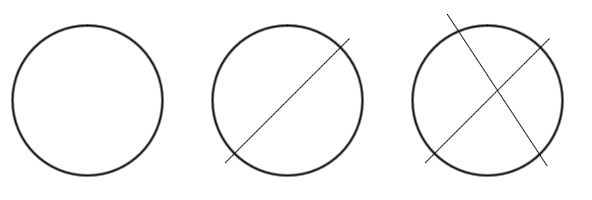
\includegraphics[scale=.45]{caterer2}}
    \end{center}
\end{figure}

{\bf Problem 2}: What is the maximum number of pieces you can cut a circular cake into with $n$ vertical cuts? Call this $c_n$.  The picture above gives the answer for $n=0,1,2$.  What is the answer for $n=3$ and $n=4$?  If you have $n-1$ cuts how many additional pieces are created by one more cut? Using the answer to the 'one more cut' questions, express $c_n$ as a recursion?  \vfill

\vfill
\end{comment}



\end{document}  